\documentclass[a4paper, 12pt]{article}

% Русский язык
\usepackage[T2A]{fontenc}
\usepackage[utf8]{inputenc}
\usepackage[english,russian]{babel}

% Картинки
\usepackage{graphicx}
\graphicspath{{images/}}
\DeclareGraphicsExtensions{.pdf,.png,.jpg}
\usepackage{wrapfig}

% Математика
\usepackage{amsmath,amsfonts,amssymb,amsthm,mathtools} 

% Параметры страницы
\usepackage[left=2cm,right=2cm,top=2cm,bottom=3cm,bindingoffset=0cm]{geometry}

\usepackage{enumitem,xparse}
\usepackage{caption}
\usepackage{subcaption}
\usepackage{float}

\begin{document}

\newgeometry{left=2cm,right=2cm,top=2cm,bottom=1cm,bindingoffset=0cm}
\begin{titlepage}
    
    \begin{center}
        \vspace*{5cm}
        \Huge Московский Физико-Технический Институт
        \vspace*{2cm}\\
        \LARGE Отчет по эксперименту
        \\\vspace*{0.25cm}
        
        \noindent\rule{\textwidth}{1pt}
        \vspace*{-0.25cm}
        
        \huge \textbf{1.1.4.\\ Изучение статистических закономерностей на примере измерения фона космического излучения}
        \noindent\rule{\textwidth}{1pt}


       \vfill
        \begin{flushright}
            \begin{minipage}{.4\textwidth}
            \Large Выполнил:\\ Студент 1 курса ФРКТ\\ Группа Б01-302 \\Хальфин Бахтияр\\
            \end{minipage}
        \end{flushright}
        
        \vfill
        \normalsize Долгопрудный \\2023
        
    \end{center}
\end{titlepage}
\restoregeometry

\setcounter{page}{2}
\section*{Аннотация}
\textbf{Цель работы:} изучить статические закономерности при измерении однородного во времени случайного процесса; проверить возможность описания интенсивности радиационного фона статистическими законами Пуассона и Гаусса; определить среднее число регистрируемых космических лучей в секунду и определить погрешность результата
\\

\noindent\textbf{В работе используются:} счетик Гейгера-Мюллера, компьютер с интерфесом для связи со счётчиком.
\\

\section*{Теоретические сведения}
\subsection*{Базовые статистические понятия}
Для простоты будем считать, что все ошибки, кроме статистических, пренебрежимо малы и рассматривать их не будем.

Наиболее важной характеристикой измерения является \textit{выборочное среднее} значение числа измерений
\begin{equation}
\langle n \rangle \equiv \frac{1}{N}\sum_{i=1}^{N} {n_i}
\end{equation}

При увеличении количества измерений, выборочное среднее будет стремиться к некоторому конечному пределу, но реальное число измерений всегда конечно, поэтому значение среднего всегда содержить \textit{погрешность}
\begin{displaymath}
\overline{n} = \lim_{N\to\infty}\langle n \rangle
\end{displaymath}

Кроме среднего значения важно знать \textit{средний квадрат отклонения}, называемый также \textit{выборочной дисперсией}

\begin{equation}
\sigma_{n}^2 \equiv \frac{1}{N}\sum_{i=1}^N{(n_i-\overline{n})^2}
\end{equation}

Аналогично при \( N \to\infty\) выборочная дисперсия стремится к некоторому предельному значению
\begin{displaymath}
    \sigma_{n}^2 = \lim_{N\to\infty}\sigma_{n}^2 = \overline{(n - \overline{n})^2}
\end{displaymath}

\textit{Погрешность среднего значения} \(\langle n \rangle\) при независимых измерениях связана со погрешность \textit{отдельного} измерения формулой

\begin{equation}\label{pogr_sr}
    \sigma_{\langle n \rangle} = \frac{\sigma_{n}}{\sqrt{N}}
\end{equation}

Таким образом, увеличивая количество измерений, среднее значение приближается к <<истинному>> \(\overline{n}\). При конечном \(N\) истинное среднее с высокой вероятностью лежит в интервале

\begin{equation}
    \overline{n} = \langle n \rangle \pm \frac{\sigma_{n}}{\sqrt{N}}
\end{equation}

\subsection*{Пуассоновский процесс}
Если события однородны во времени и каждое следующее событие не зависит от прошлого, то последовательность таких событий называют \textit{пуассоновский процессом}
Для пуассоновского процесса справедливо равенство
\begin{equation}\label{puas_osn}
    \sigma = \sqrt{\overline{n}}
\end{equation}
На практике можно ожидать приближённое равенство для \textit{выборочных} значений
\begin{displaymath}
    \sigma_{n} \approx \sqrt{\langle n \rangle}
\end{displaymath}

\subsection*{Погрешность эксперимента}
Если подставить основное свойство распределения Пуассона (\ref{puas_osn}) в формулу (\ref{pogr_sr}), получится среднеквадратичная погрешность определения среднего:
\begin{displaymath}
    \sigma_{\langle n \rangle} = \frac{\sigma_{n}}{\sqrt{N}} = \sqrt{\frac{\langle n \rangle}{N}}
\end{displaymath}
Для относительного значения погрешности:
\begin{displaymath}
    \varepsilon_{\langle n \rangle} = \frac{\sigma_{\langle n \rangle}}{\langle n \rangle} = \frac{1}{\sqrt{\langle n \rangle N}}
\end{displaymath}

\section*{Оборудование}
\begin{wrapfigure}{R}{.3\textwidth}
\centering
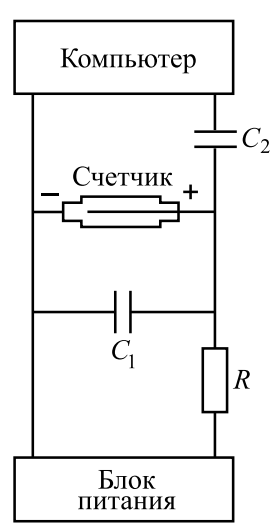
\includegraphics[width=.25\textwidth]{images/scheme.png}
\caption{Схема включения счетчика}
\end{wrapfigure}

Для измерения интенсивности космических лучей используется счетчик Гейгера-мюллера. Счеитчик представляетт собой наполненный газом сосуд с двумя электродами. Частицы космических лучей ионизируют газ, которым наполнен сосуд и выбивают электроны из его стенок. Эти электроны ускоряются электрическим полем и ионизируют молекулы газа. В результате образуется лавина электроном, и ток через счетчик резко увеличивается.

В данной работе измеряется величина, которая меняется со временем случайным образом. Методы обработки результатов те же, что и для расчет случайных погрешностей.

\noindent Погршености измерений потока частиц с помощью счетчиков Гейгера-Мюллера малы по сравнению с изменениями самого потока. Погрешности измерений определяются в основном временем, в течение которого восстанавливаются нормальные условия в счетчик после срабатывания счетчика.

В работе используется специальная компьютерная программа, с помощью которой можно получить сведения об экспериментальной установке, провести численный и реальный эксперименты.

\section*{Ход работы}

\begin{enumerate}
    \item Включаем компьютер и счетчик. В программе запускаем измерение для основного эксперимента
    \item Запускаем симуляцию с настройками по умолчанию (распределение Пуассона, интенсивность —- 1.0, ускорение -- 10). Убеждаемся, что в зависимости от количества N собранных экспериментальных точек
    \begin{enumerate}[label=\alph*)]
        \item Флуктуации среднего числа зарегистрированных частиц  $\langle n \rangle$ уменьшаются, значение выходит на постоянную величину (рис. \ref{srednee});
        \item Флуктуации среднеквадратичного отклонения $\sigma_{n}$ уменьшаются, значение выходит на постоянную величину (рис. \ref{sr_puas});
        \item $\sigma_{n}$ и $\sqrt{\langle n \rangle}$ всё больше приближаются друг к другу (рис. \ref{gistogramma_t1});
        \item Степень совпадения экспериментальной гистрограммы с теоретическими кривыми у распределения Пуассона выше, чем у распределения Гаусса (рис. \ref{gistogramma_t1}).
    \end{enumerate}
\end{enumerate}

\begin{figure}[H]
\centering
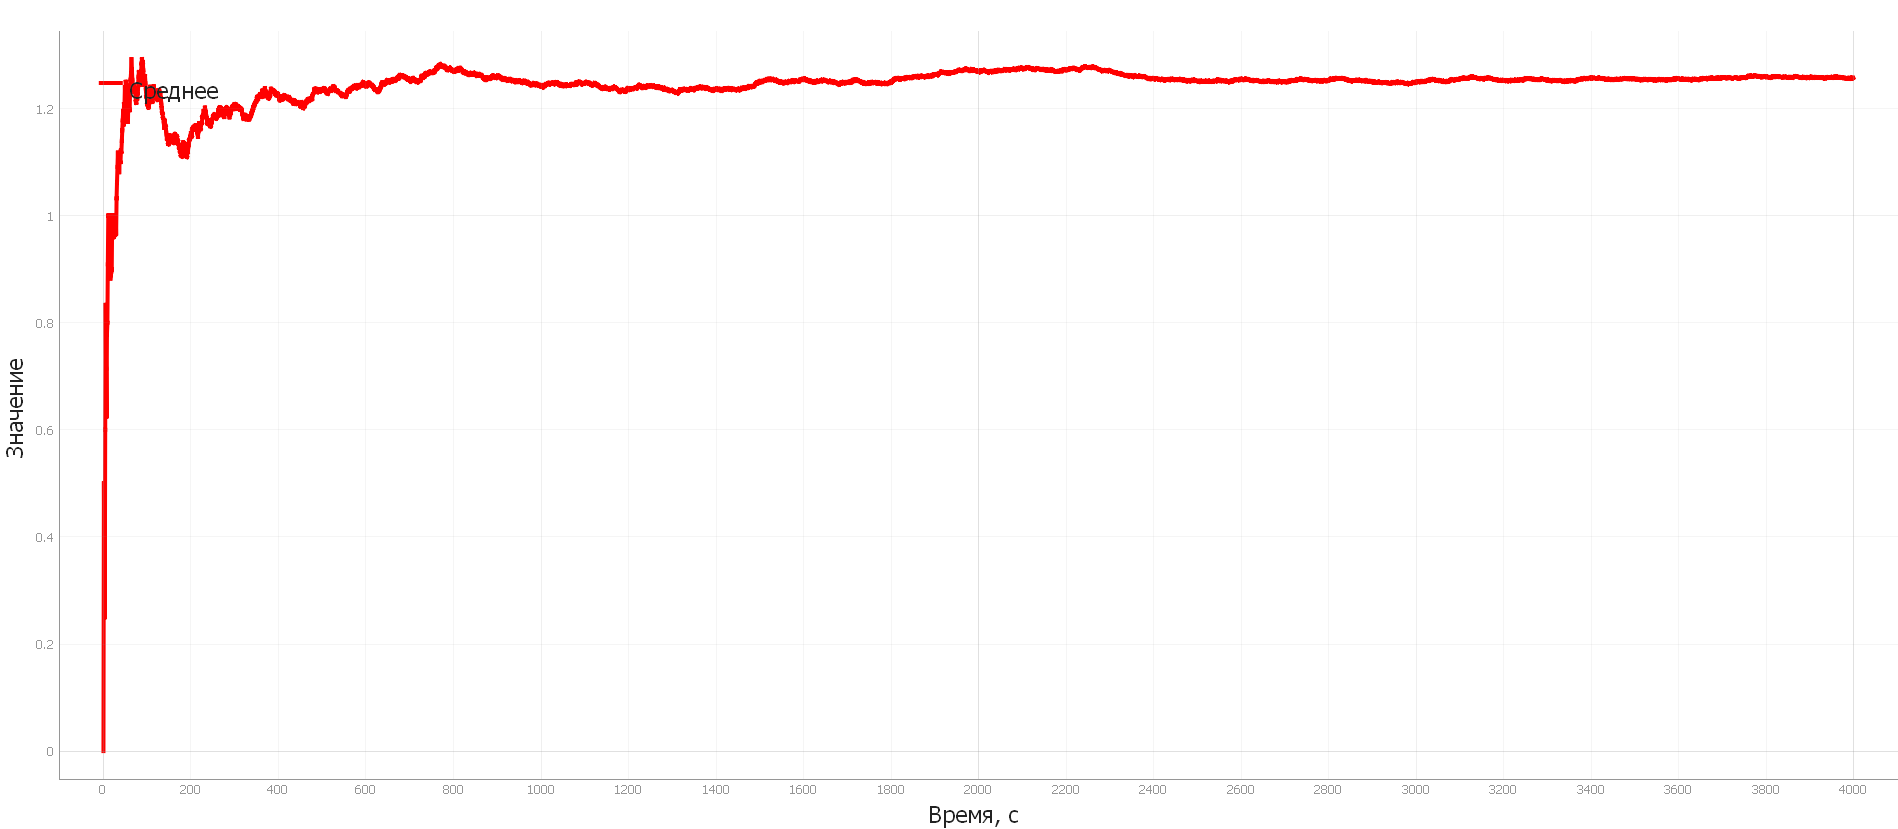
\includegraphics[width=1\linewidth]{images/experiment_graph_02.png}
\caption{Среднее число зарегистрированных частиц}
\label{srednee}
\end{figure}

\begin{figure}[H]
\centering
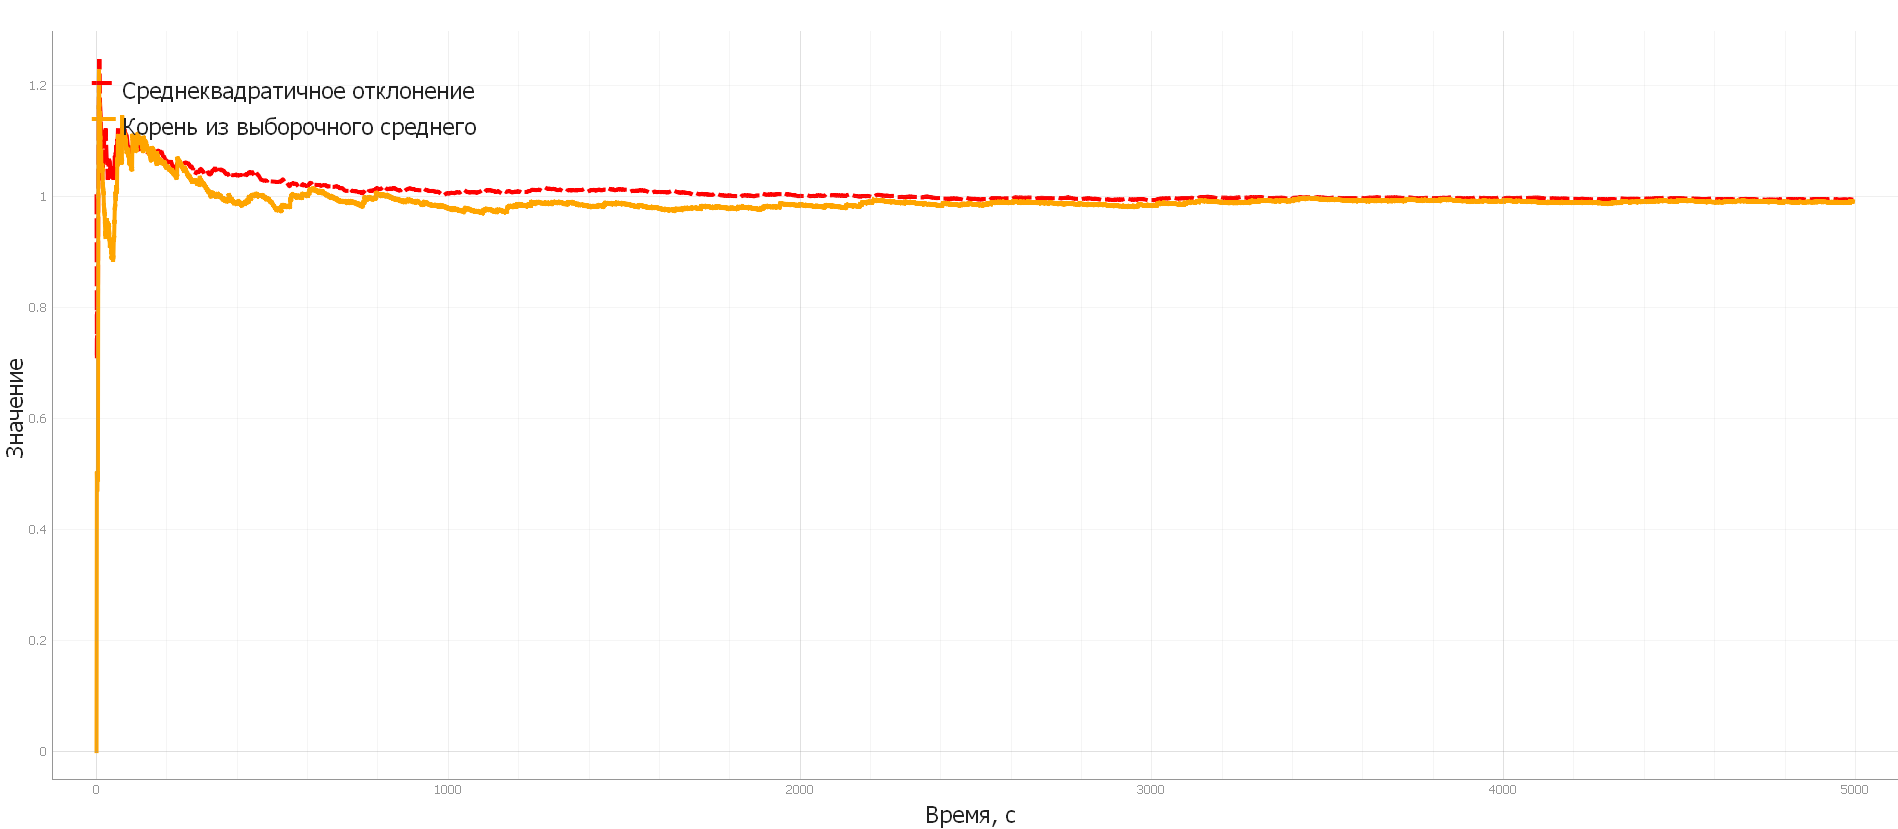
\includegraphics[width=1\linewidth]{images/sr_puas.png}
\caption{Среднее квадратичное значение и корень из выборочного среднего}
\label{sr_puas}
\end{figure}

\begin{figure}[H]
\centering
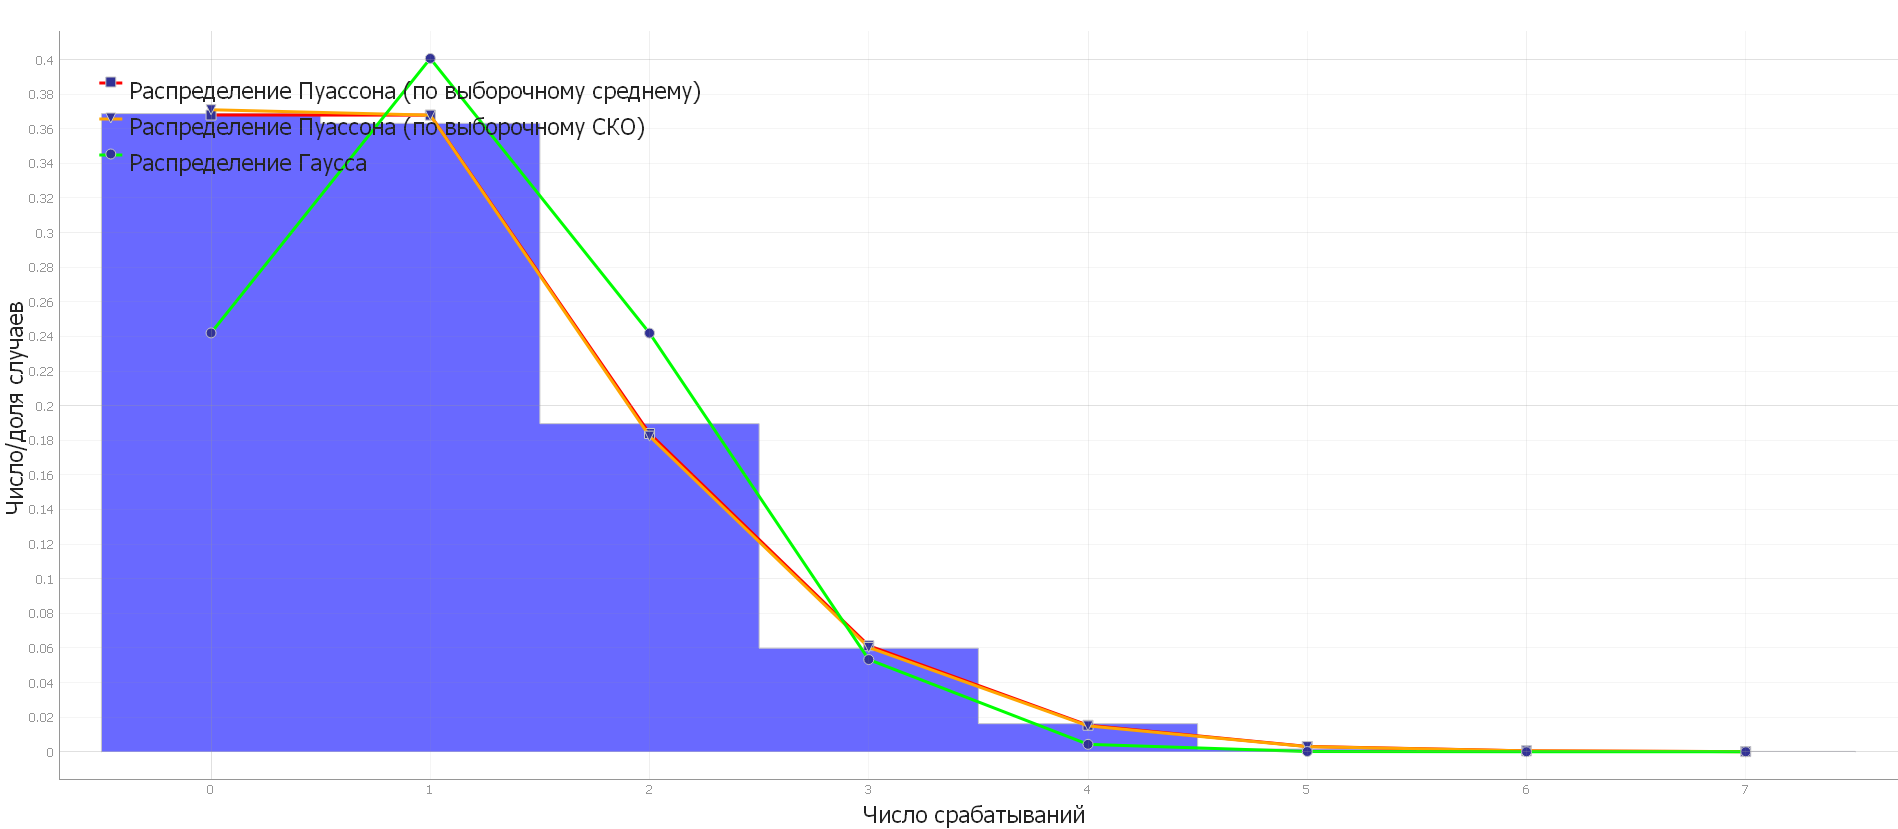
\includegraphics[width=1\linewidth]{images/t_1.png}
\caption{Гистограмма}
\label{gistogramma_t1}
\end{figure}

3. Рассмотрим как изменяются гистограммы для параметра группировки результатов $\tau$ = 10; 20; 80:
\begin{figure}[H]
\captionsetup[subfigure]{labelformat=empty}
\centering
\begin{subfigure}{.33\textwidth}
    \centering
    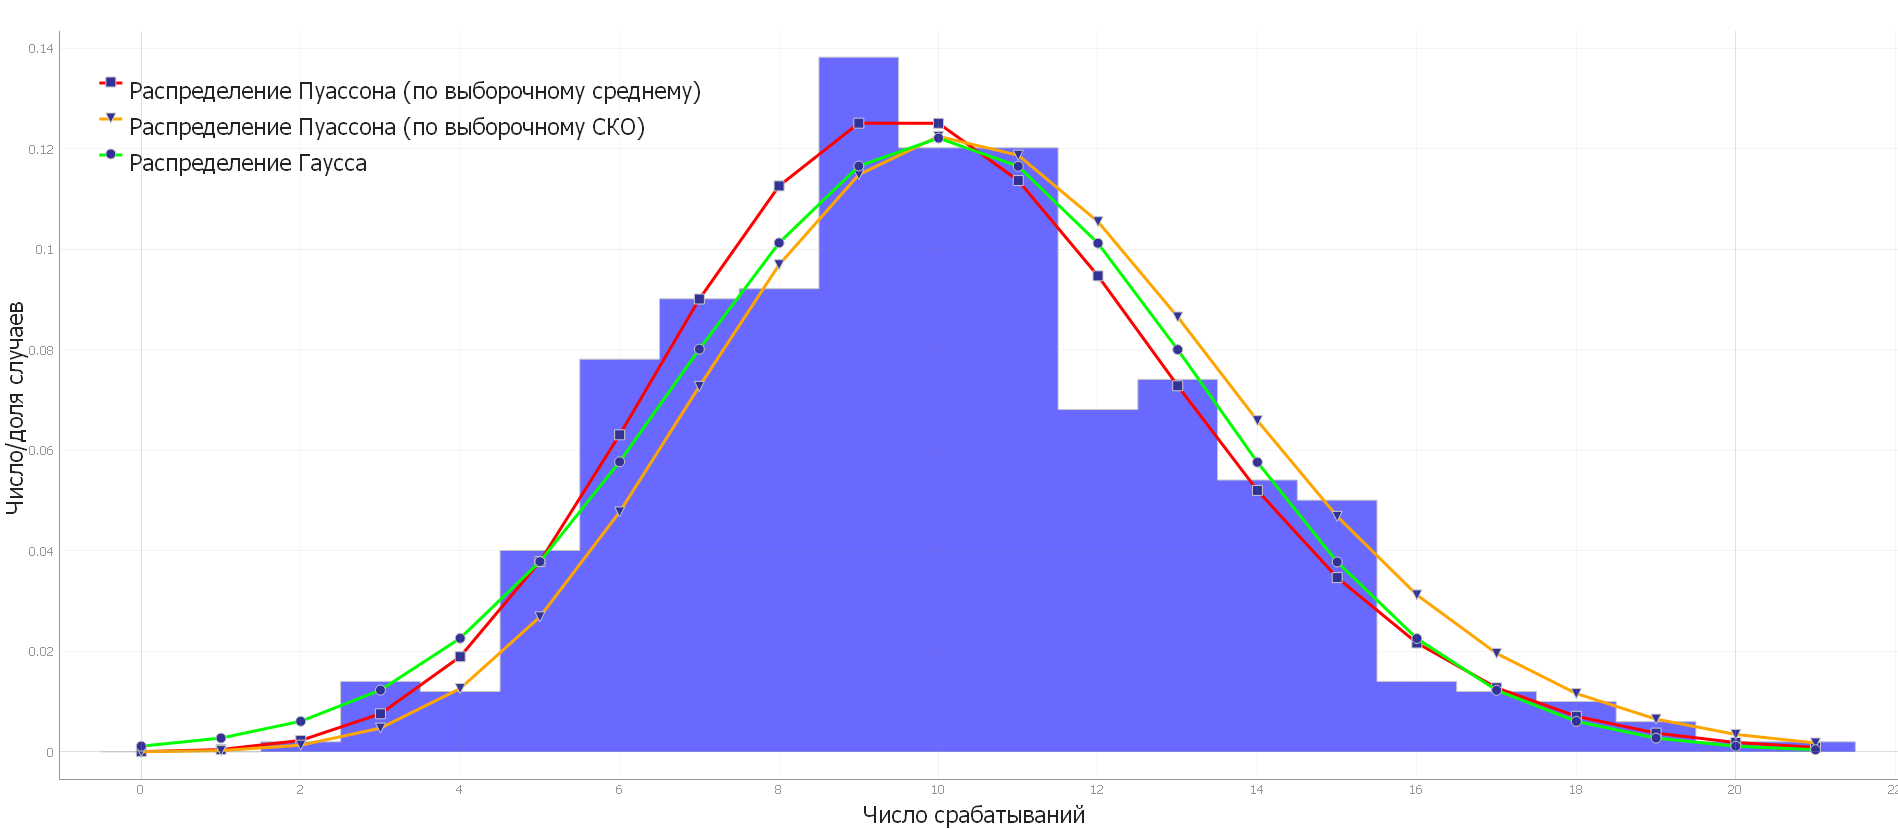
\includegraphics[width=1\linewidth]{t_10}
    \caption{$\tau$ = 10}
\end{subfigure}%
\begin{subfigure}{.33\textwidth}
    \centering
    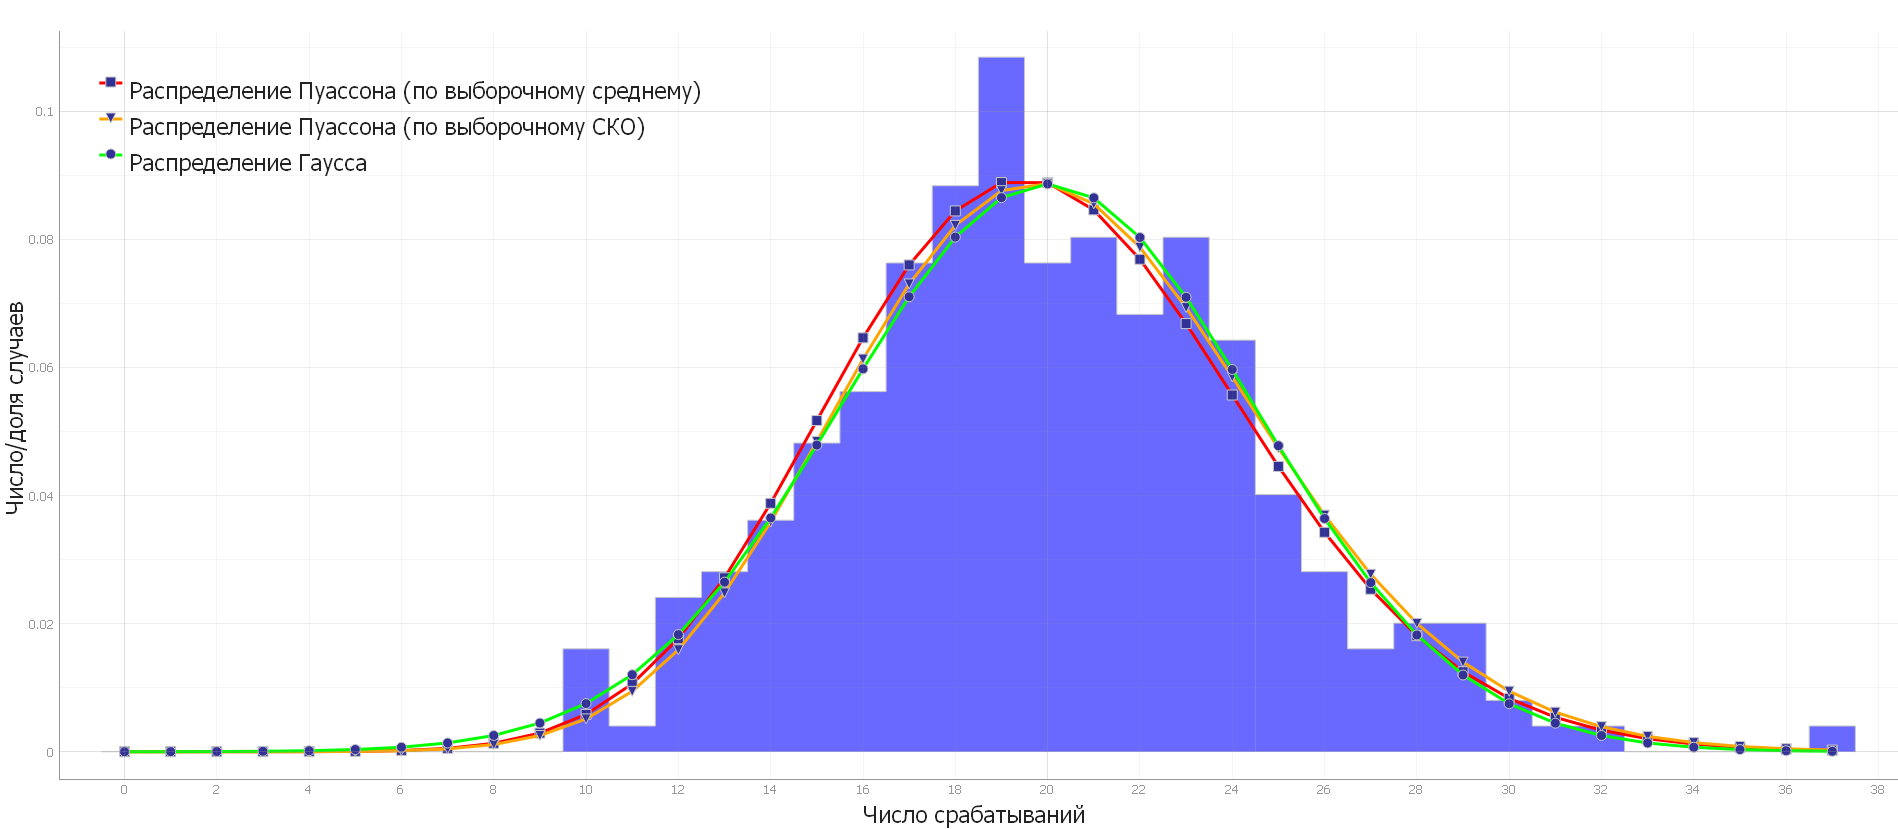
\includegraphics[width=1\linewidth]{t_20}
    \caption{$\tau$ = 20}
\end{subfigure}%
\begin{subfigure}{.33\textwidth}
    \centering
    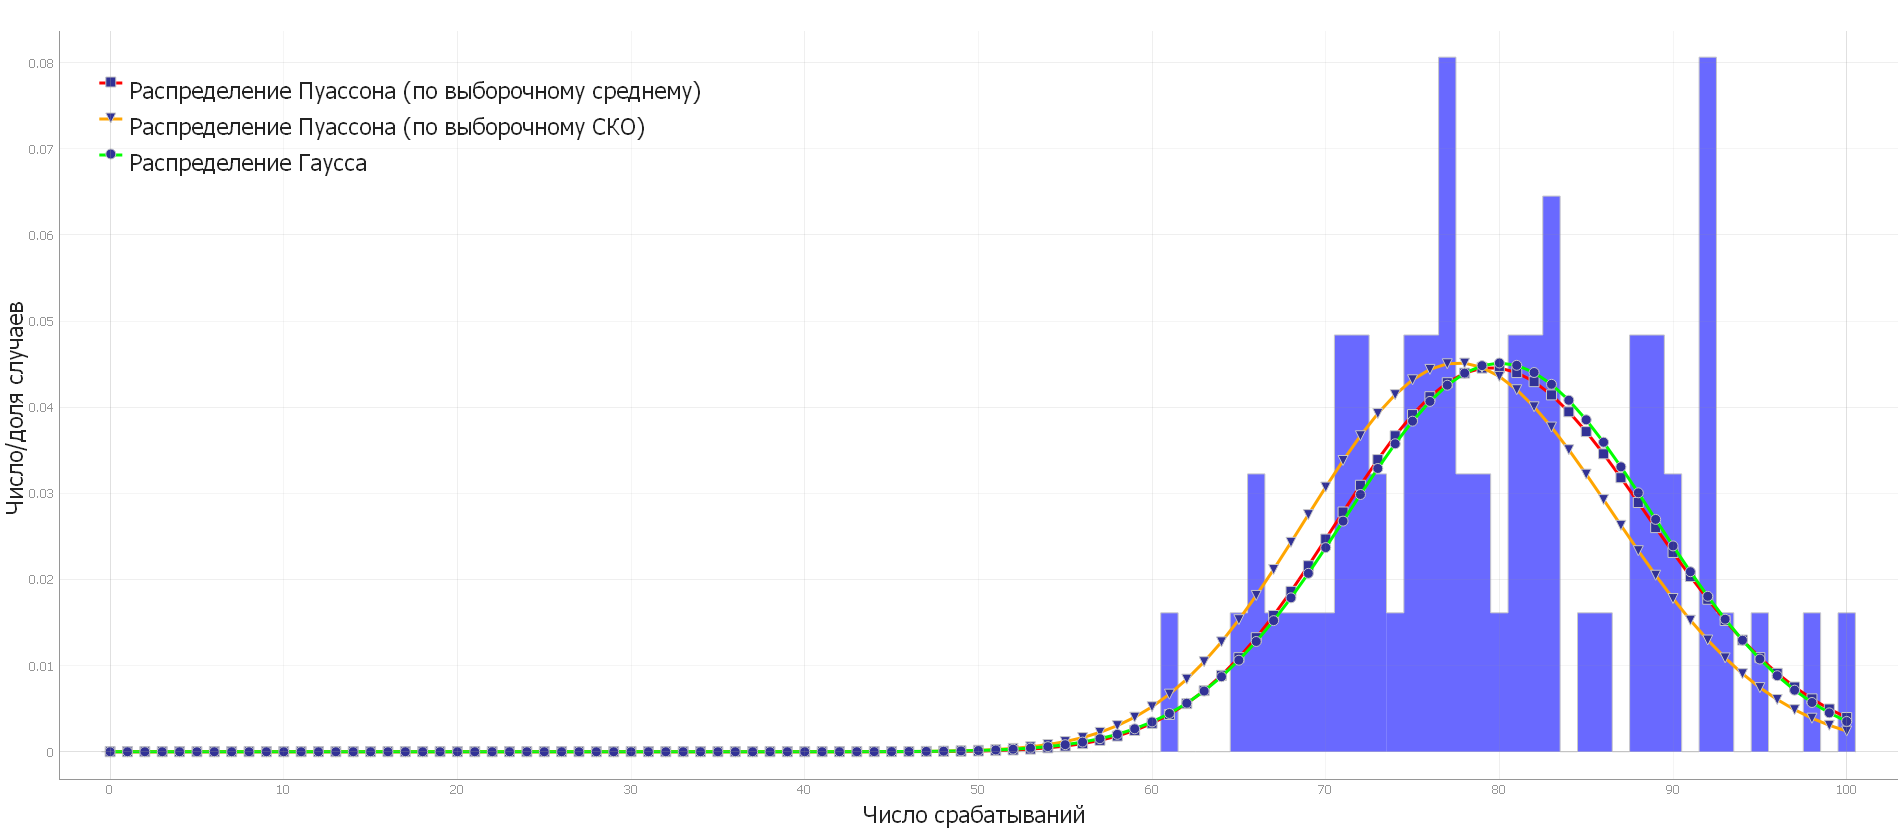
\includegraphics[width=1\linewidth]{t_80}
    \caption{$\tau$ = 80}
\end{subfigure}
\end{figure}

При изменении порядка группировки результатов $\tau$ максимальная доля случаев уменьшается (в силу увеличения количества групп). График распределения Гаусса и Пуассона принимает более округлый вид.


4. Рассмотрим как изменяются гистограммы для параметра средней интенсивности числа частиц $\mu$ = 2; 4; 10; 25.
\begin{figure}[H]
\captionsetup[subfigure]{labelformat=empty}
\centering
\begin{subfigure}{.25\textwidth}
    \centering
    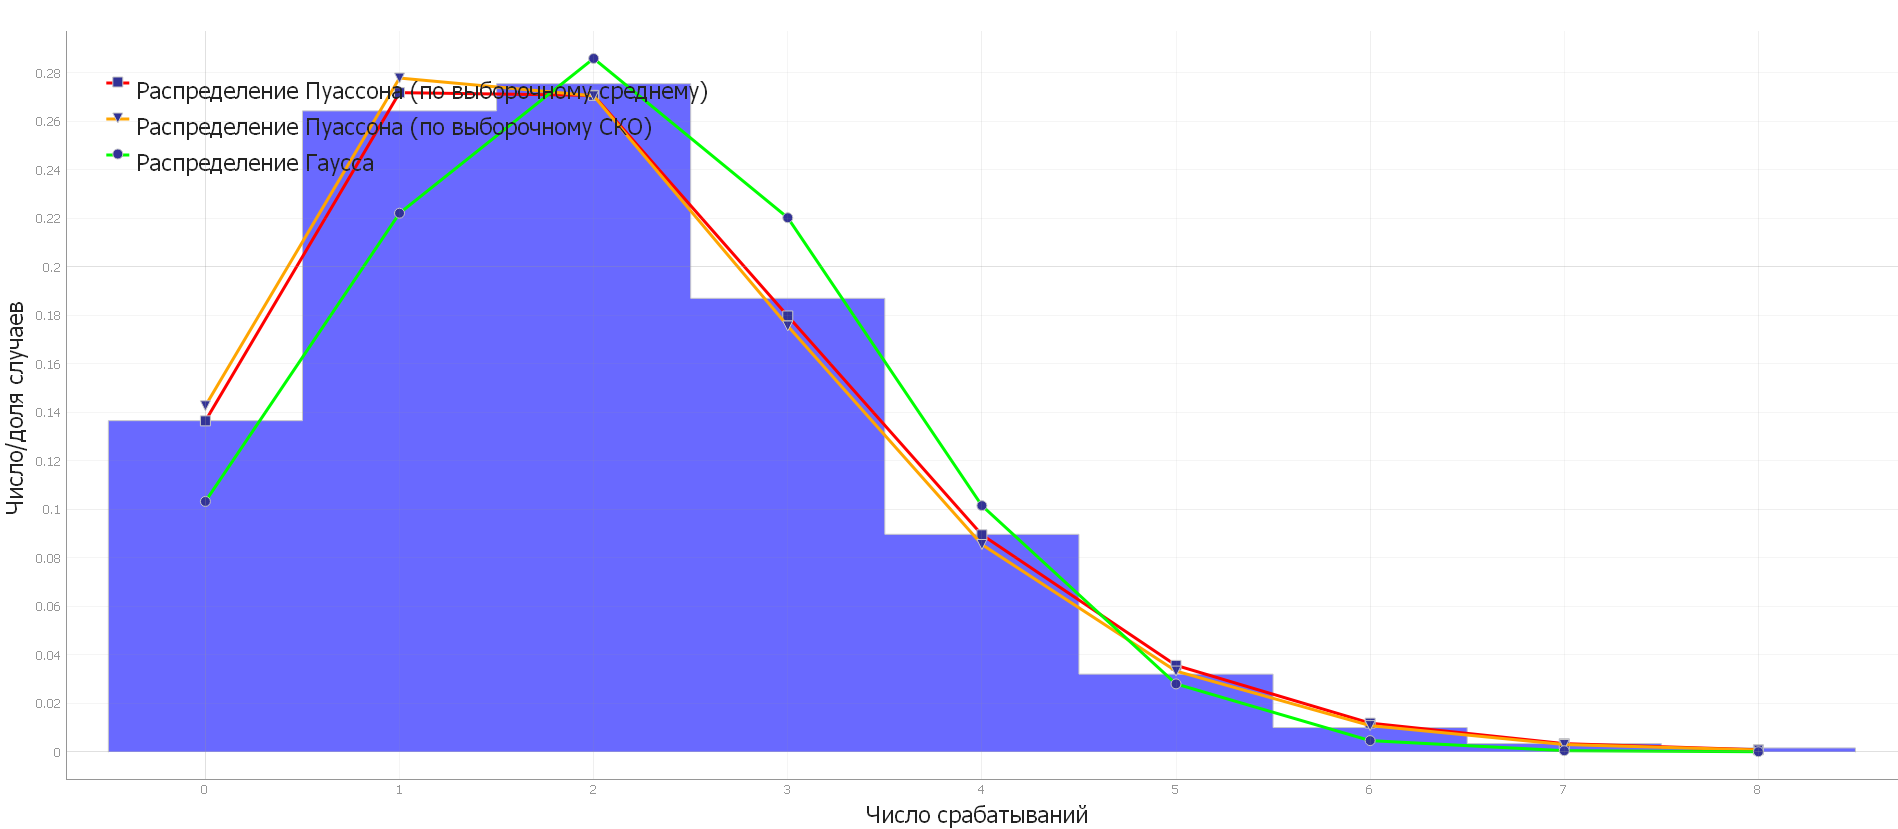
\includegraphics[width=1\linewidth]{m_2}
    \caption{$\mu$ = 2}
\end{subfigure}%
\begin{subfigure}{.25\textwidth}
    \centering
    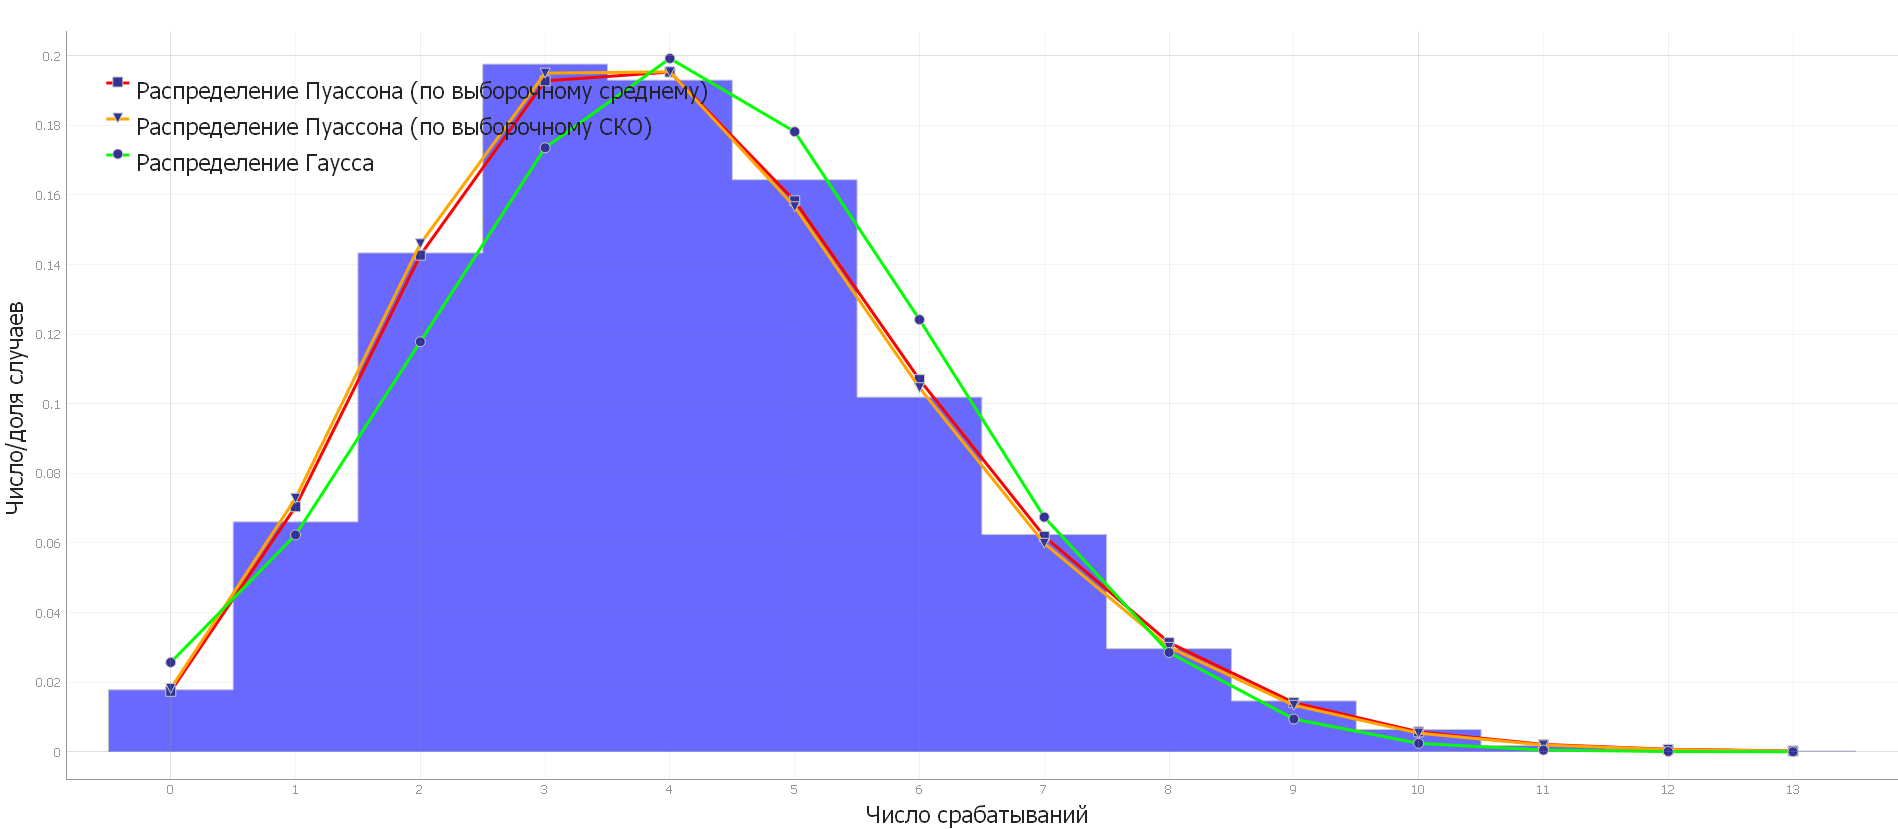
\includegraphics[width=1\linewidth]{m_4}
    \caption{$\mu$ = 4}
\end{subfigure}%
\begin{subfigure}{.25\textwidth}
    \centering
    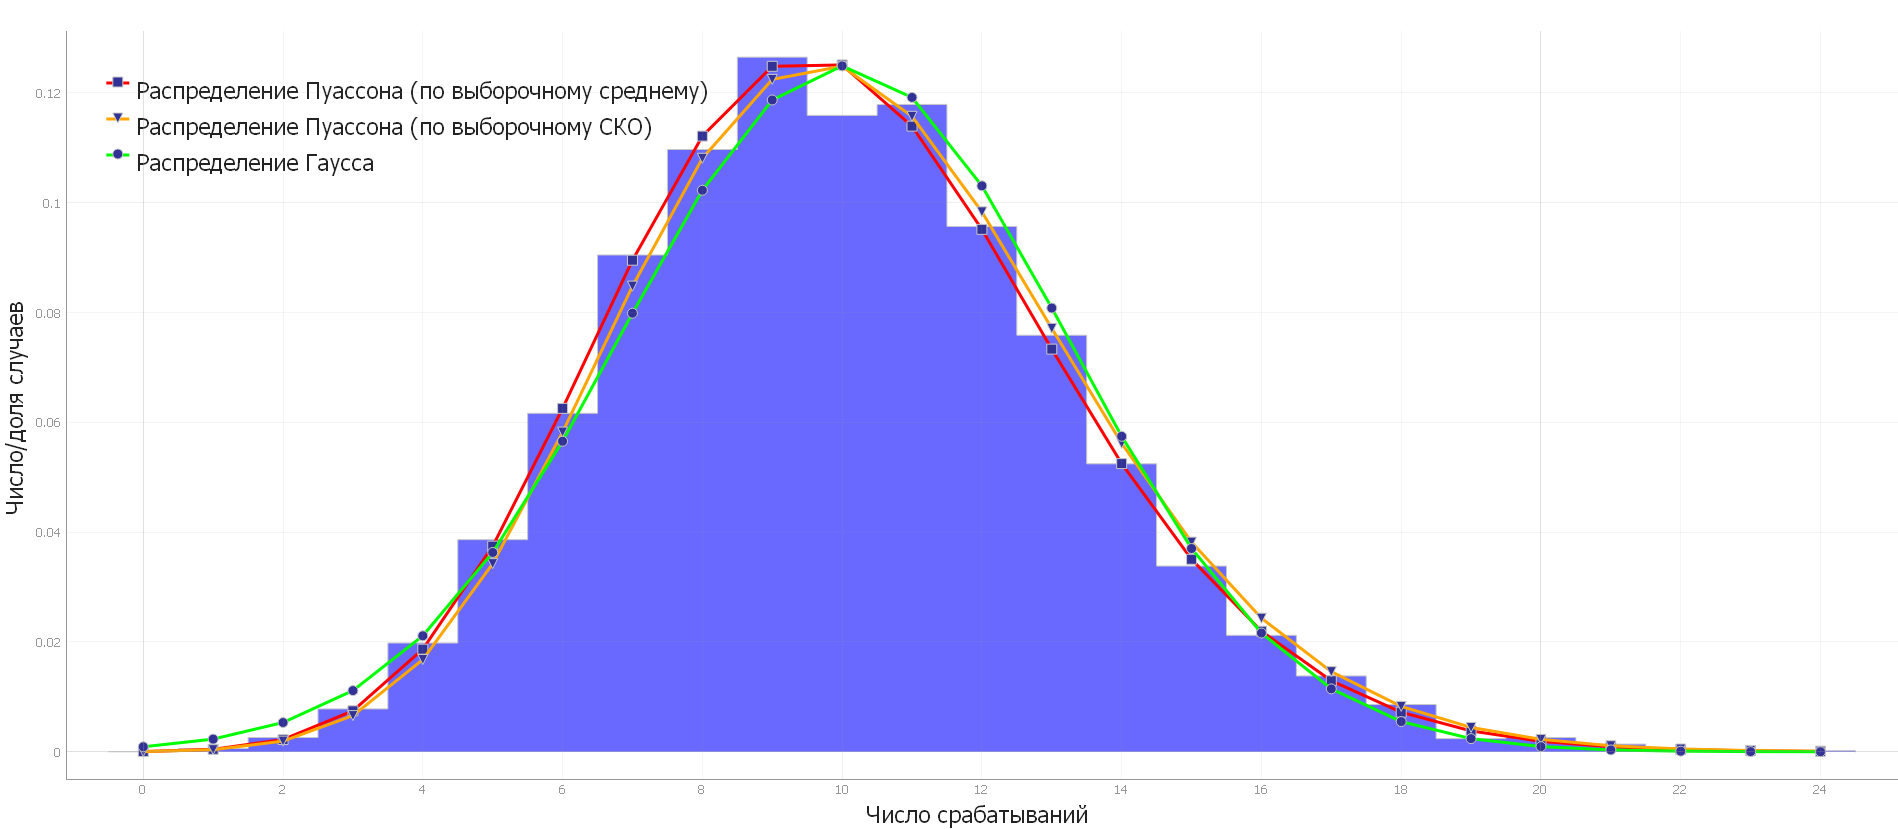
\includegraphics[width=1\linewidth]{m_10}
    \caption{$\mu$ = 10}
\end{subfigure}%
\begin{subfigure}{.25\textwidth}
    \centering
    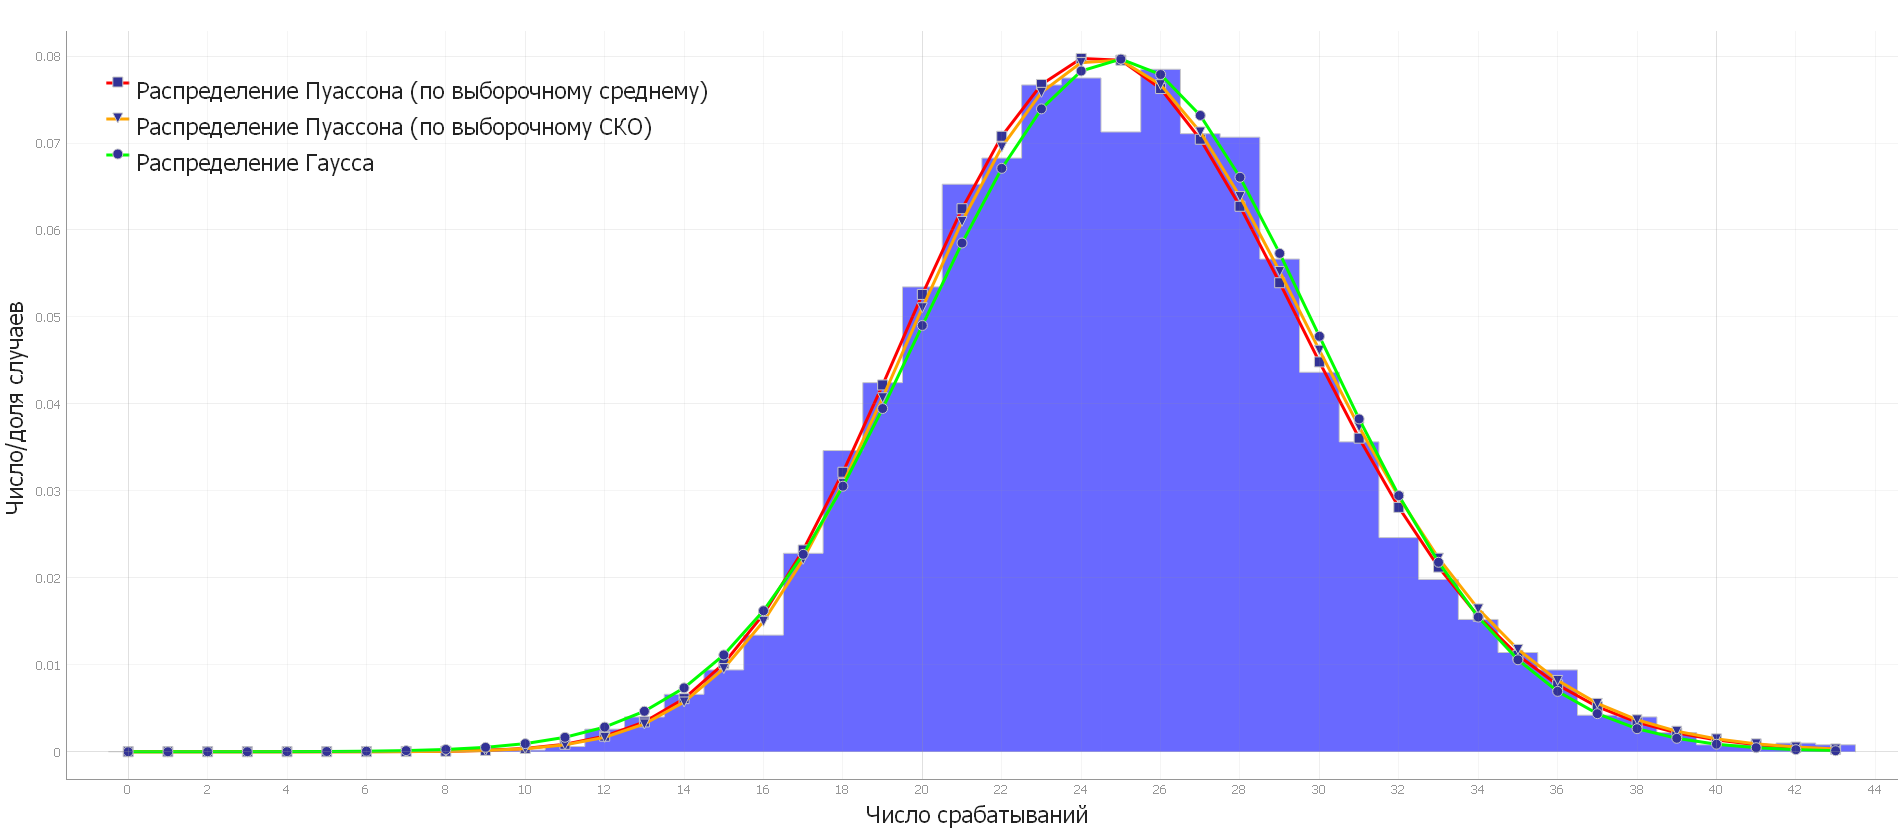
\includegraphics[width=1\linewidth]{m_25}
    \caption{$\mu$ = 25}
\end{subfigure}
\end{figure}

При изменении порядка группировки результатов $\mu$ максимальная доля случаев уменьшается (в силу увеличения количества групп). График распределения Гаусса и Пуассона принимает более округлый вид.

\section*{Обработка результатов}
Для основного эксперимента сгруппируем данные с различными интервалами группировки $\tau$ = 10с; 20с; 40с; 80с.

\begin{figure}[H]
\centering
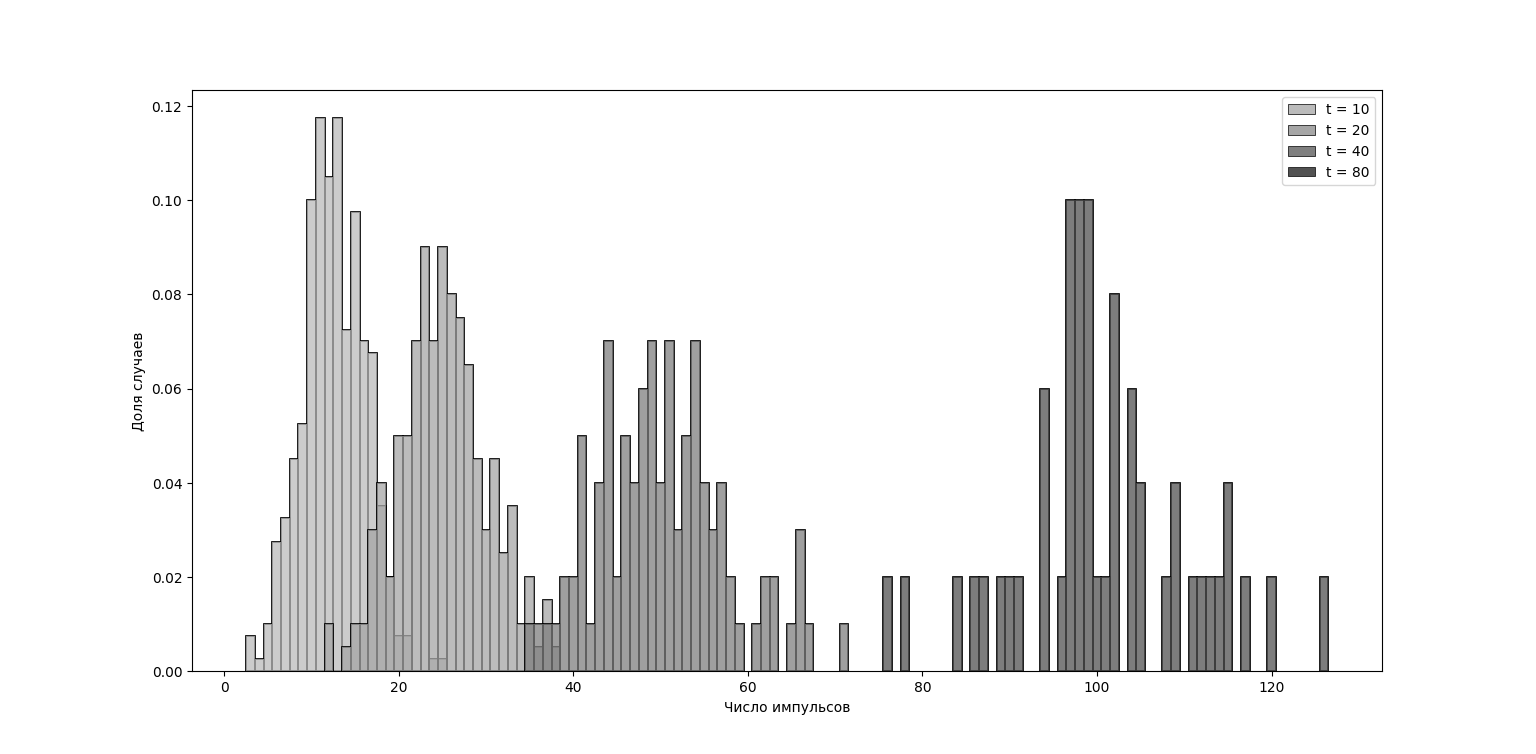
\includegraphics[width=1\linewidth]{images/Figure_1.png}
\caption{Гистограмма для числа отсчетов $n$ и $w_{n}$}
\end{figure}

Для каждого $\tau$ вычислим средее число регистрируемых частиц $\langle n \rangle$:
\begin{equation*}
  \begin{aligned}
    \langle n_{10} \rangle = \frac{1}{N}\sum_{i=1}^{N} {n_i} \approx 10.09\\    
    \langle n_{20} \rangle = \frac{1}{N}\sum_{i=1}^{N} {n_i} \approx 20.18\\
    \langle n_{40} \rangle = \frac{1}{N}\sum_{i=1}^{N} {n_i} \approx 40.36\\
    \langle n_{80} \rangle = \frac{1}{N}\sum_{i=1}^{N} {n_i} \approx 80.72
  \end{aligned}
\end{equation*}


Для каждого $\tau$ вычислим среднеквадратичное отклонение $\sigma_{n}$:  

\begin{equation*}
  \begin{aligned}
        \sigma_{n_{10}} = \sqrt{\frac{1}{N}\sum_{i=1}^N{(n_i-\overline{n})^2}} \approx 3.14\\
        \sigma_{n_{20}} = \sqrt{\frac{1}{N}\sum_{i=1}^N{(n_i-\overline{n})^2}} \approx 4.39\\
        \sigma_{n_{40}} = \sqrt{\frac{1}{N}\sum_{i=1}^N{(n_i-\overline{n})^2}} \approx 6.40\\
        \sigma_{n_{80}} = \sqrt{\frac{1}{N}\sum_{i=1}^N{(n_i-\overline{n})^2}} \approx 9.91
  \end{aligned}
\end{equation*}

Для каждого $\tau$ вычислим погрешность среднего значения $\sigma_{\langle n \rangle}$:  

\begin{equation*}
  \begin{aligned}
        \sigma_{\langle n_{10} \rangle} = \frac{\sigma_{n}}{\sqrt{N}} \approx 0.16\\ 
        \sigma_{\langle n_{20} \rangle} = \frac{\sigma_{n}}{\sqrt{N}} \approx 0.31\\
        \sigma_{\langle n_{40} \rangle} = \frac{\sigma_{n}}{\sqrt{N}} \approx 0.64\\
        \sigma_{\langle n_{80} \rangle} = \frac{\sigma_{n}}{\sqrt{N}} \approx 1.40 
  \end{aligned}
\end{equation*}


\newpage
Для каждого $\tau$ вычислим среднюю интенсивность регистрируемых частиц в секунду $j$:  
\begin{gather*}
    \langle j_{10} \rangle = \frac{\langle n \rangle}{\tau} \approx 1.01\\ 
    \sigma_{\langle 10 \rangle} = \frac{\sigma_{n}}{\tau} =  \approx 0.02\\
    \overline{j_{10}} = \langle j_{10} \rangle \pm \frac{\sigma_{j_{10}}}{\sqrt{N}} = 1.01 \pm 0.016
    \langle j_{20} \rangle = \frac{\langle n \rangle}{\tau} \approx 1.01\\ 
    \sigma_{\langle 20 \rangle} = \frac{\sigma_{n}}{\tau} =  \approx 0.016\\
    \overline{j_{20}} = \langle j_{20} \rangle \pm \frac{\sigma_{j_{20}}}{\sqrt{N}} = 1.01 \pm 0.016 
    \langle j_{40} \rangle = \frac{\langle n \rangle}{\tau} \approx 1.01\\ 
    \sigma_{\langle 40 \rangle} = \frac{\sigma_{n}}{\tau} =  \approx 0.016\\
    \overline{j_{40}} = \langle j_{40} \rangle \pm \frac{\sigma_{j_{40}}}{\sqrt{N}} = 1.01 \pm 0.016
        \langle j_{80} \rangle = \frac{\langle n \rangle}{\tau} \approx 1.01\\ 
    \sigma_{\langle 80 \rangle} = \frac{\sigma_{n}}{\tau} =  \approx 0.016\\
    \overline{j_{80}} = \langle j_{80} \rangle \pm \frac{\sigma_{j_{80}}}{\sqrt{N}} = 1.01 \pm 0.016
\end{gather*}

Можно заметить, что средняя интенсивность регистрируемых частиц в секунду не зависит от величины интервала $\tau$ и числа точек $N = t / \tau$

Наложим поверх экспериментальных гистограмм теоретические распределения Пуассона и Гаусса.
\begin{figure}[H]
\centering
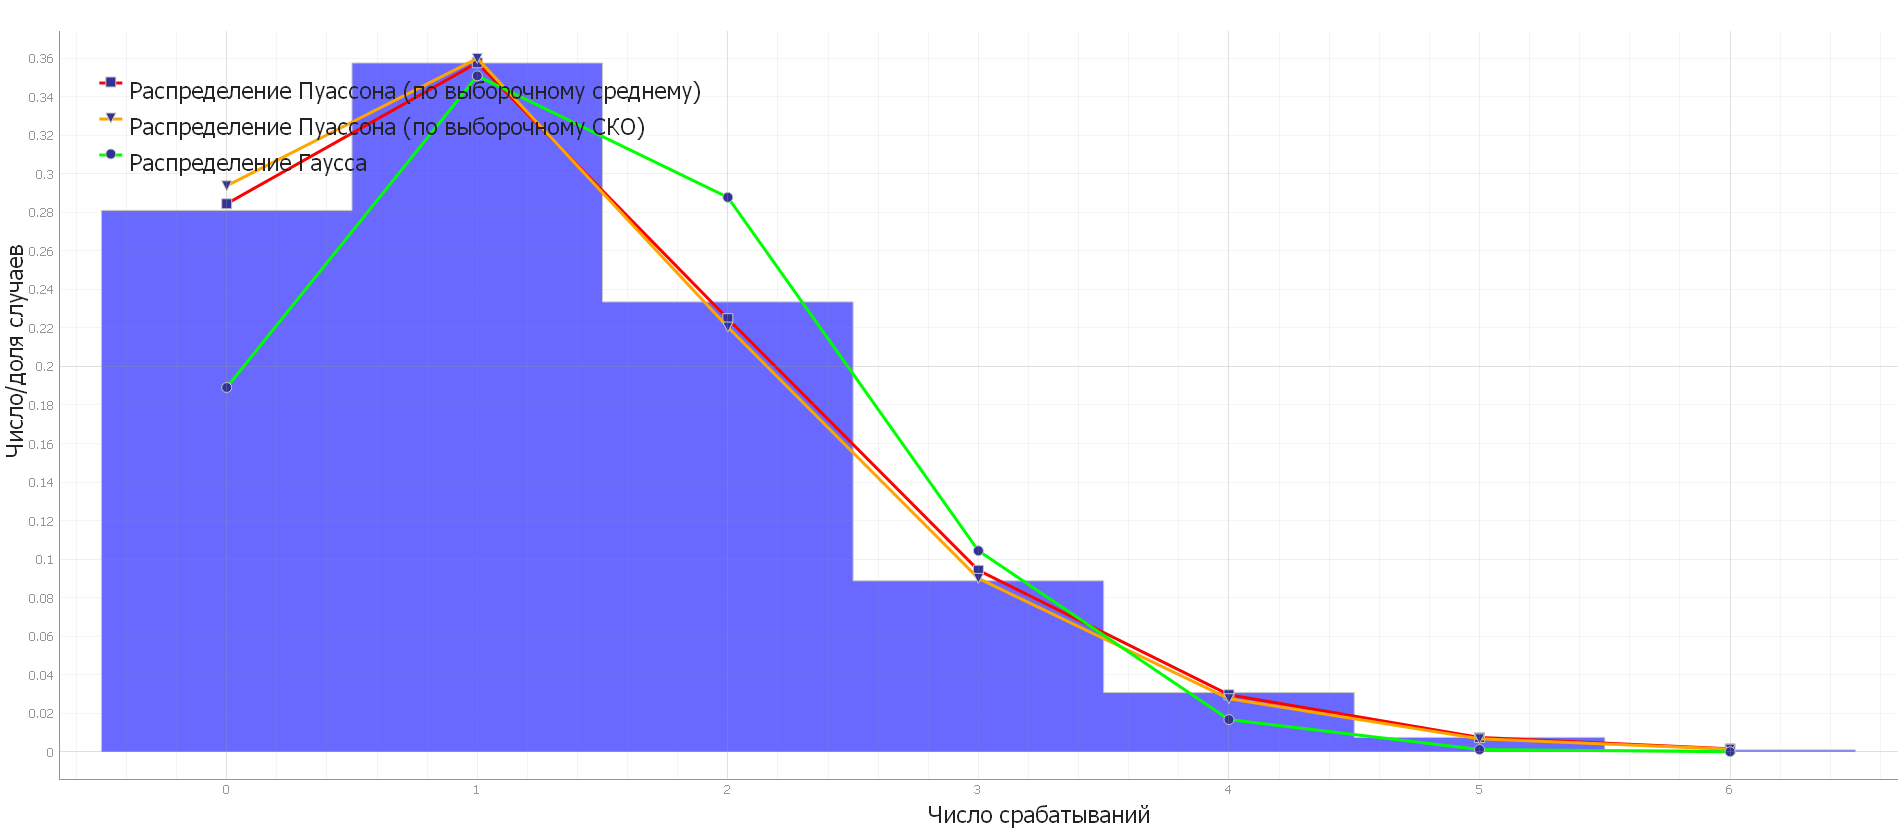
\includegraphics[width=1\linewidth]{images/experiment_graph_01.png}
\caption{Гистограмма с наложенными распределениями Пуассона и Гаусса}
\end{figure}

Экспериментальные гистограммы с большой точностью согласуются с распределениями Пуассона и с несколько меньшей точностью с распределением Гаусса.

Проверим справедливость основного свойства распределения Пуассона
\begin{gather*}
\sqrt{\langle n \rangle} \approx \sigma_n\\
\sqrt{10.09} \approx 3.18  \approx 3.14
\end{gather*}
Данное равенство выполняется с точностью до десятых. Можно сделать вывод, что регистрация частиц является однородным во времени случайным процессом, а количество отсчётов в одном опыте подчиняется распределению Пуассона.

Определим доли случаев, когда отклонение числа отсчётов $n$ от среднего значения не превышает (по модулю) одного, двух и трёх стандартных отклонений:
\begin{gather*}
|n - \langle n \rangle| \leq \sigma_n\\
w_1 = 0.59\\
|n - \langle n \rangle| \leq 2\sigma_n\\
w_2 = 0.96\\
|n - \langle n \rangle| \leq 3\sigma_n\\
w_3 = 0.99
\end{gather*}

\noindentСравним результаты с теоретическими для распределния Гаусса:
\begin{gather*}
|n - \langle n \rangle| \leq \sigma_n\\
w_1 = 0.67\\
|n - \langle n \rangle| \leq 2\sigma_n\\
w_2 = 0.93\\
|n - \langle n \rangle| \leq 3\sigma_n\\
w_3 = 0.99
\end{gather*}
Можно сделать вывод, что при достаточно больших $\overline{n}$ распределение Пуассона приближается к \textit{нормальному распределению (распределению Гаусса)}
\section*{Вывод}
В ходе выполнения работы познакомился с основными понятиями статистики. Определил среднее число регистрируемых космических лучей в секунду и определил погрешность результата. Выяснил, что средняя интенсивность регистрируемых частиц в секунду не зависит от величины интервала $\tau$ и числа точек $N = t / \tau$. Проверил возможность описания исследуемого процесса статистическими законами Пуассона и Гаусса.
\end{document}
